%%%%%%%%%%%%%%%%%%%%%%%%%%%%%%%%%%%%%%%%%%%%%%%
% University Paderborn Beamer Presentation 

% Author: Ashwin Prasad Shivarpatna Venkatesh 

%This template is free: you can redistribute it and/or modify
%it under the terms of the GNU General Public License as published by
%the Free Software Foundation, either version 3 of the License, or any later version.
%
%This program is distributed in the hope that it will be useful,
%but WITHOUT ANY WARRANTY; without even the implied warranty of
%MERCHANTABILITY or FITNESS FOR A PARTICULAR PURPOSE.  See the
%GNU General Public License for more details.
%
%You should have received a copy of the GNU General Public License
%along with this program.  If not, see <https://www.gnu.org/licenses/>.

%%%%%%%%%%%%%%%%%%%%%%%%%%%%%%%%%%%%%%%%%%%%%%%

\documentclass{beamer}
% Default page size 12.8cm x 9.6cm

% import packages and user-defined commands
\usepackage{amsmath, amssymb, amsfonts}% mathematical symbols and the like
\usepackage{amsthm}% definitions, theorems, etc.
\usepackage[colorinlistoftodos]{todonotes}% marking open todos in text/on margins
\usepackage{subfig}% multi-part figures with separate captions per part
\usepackage{url}% render URLs correctly and make them clickable through the hyperref package
\usepackage{longtable}% tables that span multiple pages
\usepackage{booktabs}% tables that actually look good
\usepackage[nolist]{acronym}% consistently use acronyms
\usepackage{caption}
\usepackage{graphicx}
%%%%%%%%%
% Some commands for setting up theorem environments as provided by package 
% amsthm --- language sensitive
%%%%%%%%%
\theoremstyle{plain}
\newtheorem{definition}{Definition}[chapter]
\newtheorem{lemma}[definition]{Lemma}
\ifgerman
	\newtheorem{theorem}[definition]{Satz}
	\newtheorem{corollary}[definition]{Korollar}
	\newtheorem{example}[definition]{Beispiel}
\else
	\newtheorem{theorem}[definition]{Theorem}
	\newtheorem{corollary}[definition]{Corollary}
	\newtheorem{example}[definition]{Example}
\fi


%%%%%%%%%
% Your commands should go here...
%%%%%%%%%
\newcommand*{\eg}{e.\,g.}
\newcommand*{\ie}{i.\,e.}
\newcommand*{\cf}{c.\,f.}
\newcommand*{\etal}{et~al.}

\newcommand{\code}[1]{\texttt{#1}\xspace}

\newacro{template}[UPB-CS-TT]{Paderborn University Computer Science thesis template}

\DeclareMathOperator{\testop}{top}




\definecolor{uni-blue}{cmyk}{1.0, 0.85, 0.05, 0.36, 1.00}
\definecolor{uni-cyan}{cmyk}{0.72, 0.08, 0.0, 0.0, 1.00}
\definecolor{uni-green}{cmyk}{0.50, 0.0, 0.95, 0.0, 1.00}
\definecolor{uni-orange}{cmyk}{0.0, 0.50, 0.95, 0.0, 1.00}
\definecolor{uni-purple}{cmyk}{0.38, 0.88, 0.08, 0.0, 1.00}
\definecolor{uni-gray}{cmyk}{0.0, 0.0, 0.0, 0.30}
\definecolor{uni-black}{cmyk}{0.0, 0.0, 0.0, 0.80}

\setbeamertemplate{navigation symbols}{}
\setbeamercolor{structure}{fg=uni-blue} % itemize, enumerate, etc
\setbeamercolor{normal text}{fg=uni-black}

\setbeamercolor{section in toc}{fg=uni-blue} % TOC sections
\setbeamercolor{subsection in toc}{fg=uni-black} % TOC sections

\setbeamertemplate{subsection  in toc}[square]
\setbeamertemplate{section in toc}[circle]

\setbeamerfont{section number projected}{size=\large}
\setbeamercolor{section number projected}{bg=uni-blue,fg=white}
\setbeamercolor{subsection number projected}{bg=uni-black,fg=white}

% Universal background except title
\usebackgroundtemplate{%
	
\includegraphics[width=\paperwidth,height=\paperheight]{images/otherbackground.pdf}} 

%----------------------------------------------------------------------------------------
%	FOOTER THEME
%----------------------------------------------------------------------------------------

\setbeamertemplate{footline}[text line]{%
		
	\setbeamercolor{footline}{bg=,fg=uni-blue}	
	
	\begin{beamercolorbox}[sep=0.3cm,ht=2.6em,wd=\paperwidth]{footline}
		
		\vbox{}\vskip-2ex%
		\hspace{0.0cm}
		\insertshortauthor
		\hfill
		\fontfamily{phv}\fontseries{bc}\selectfont\bfseries 
		\insertframenumber
		\hfill
		\vskip-0.8ex%
	\end{beamercolorbox}
	
}

%----------------------------------------------------------------------------------------
%	ITEMIZE CIRCLE
%----------------------------------------------------------------------------------------

\setbeamertemplate{itemize items}{
	\begin{tikzpicture}
	\node[circle, draw, semithick, inner sep=0pt, minimum size=4pt] (1) at (0,0) {};
	\end{tikzpicture}
}

%----------------------------------------------------------------------------------------
%	TITLE PAGE
%----------------------------------------------------------------------------------------

\setbeamertemplate{title page}{%

	\begin{tikzpicture}[remember picture,overlay]
	
	% Uni logo
	\node[inner sep=0pt] (logo) at (1.1, 3)
	{
\includegraphics[width=.3\textwidth]{images/logo.pdf}};
	
	% Uni pic
	\node[inner sep=0pt] (logo) at (9.175, 1.62)
	{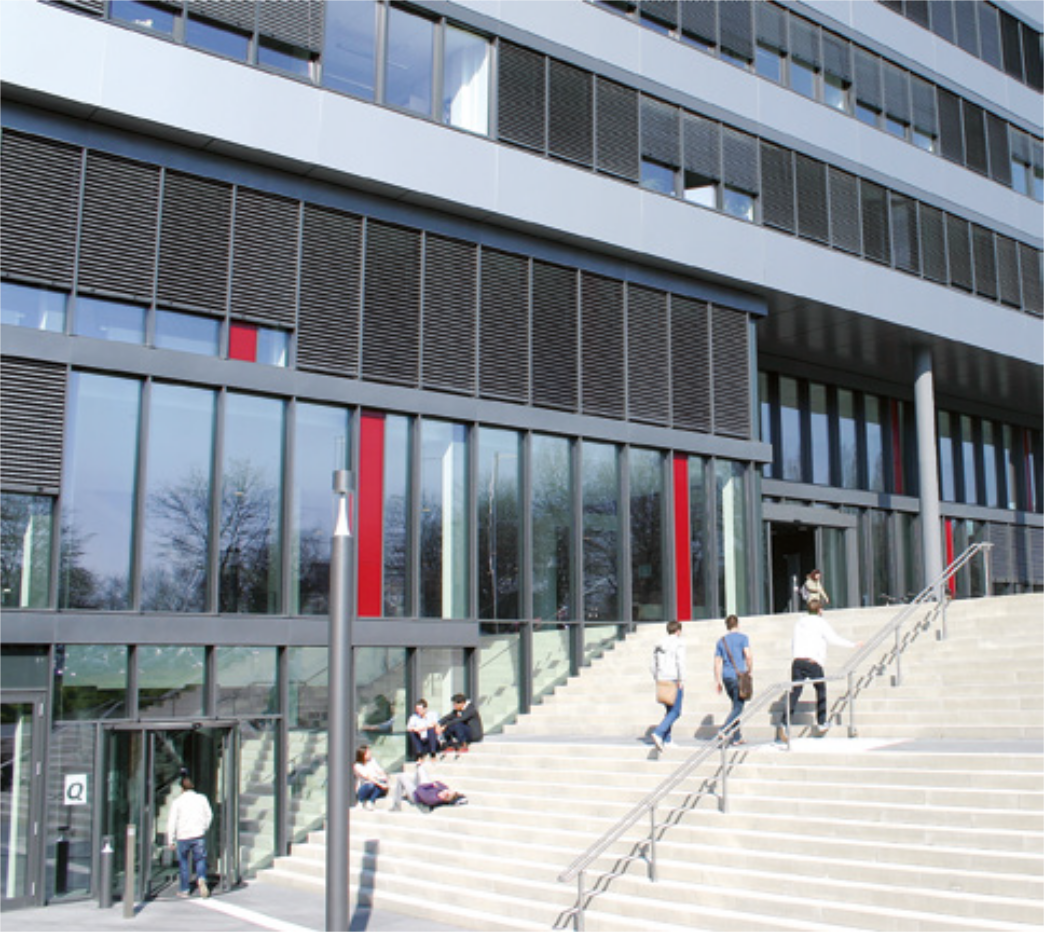
\includegraphics[width=.485\textwidth]{images/unibuilding.png}};
	

	\node[inner sep=0pt] (tit) at (4.40, -2.7)
	{
		\begin{minipage}[t]{1.0\linewidth} 
		\setbeamercolor{title}{bg=\upbcolor,fg=white}	
		
		\begin{minipage}[t]{1.0\linewidth} 
		\setbeamercolor{title}{bg=,fg=uni-blue}	
		\begin{beamercolorbox}[sep=2pt,left]{title}
		{\hspace{4pt}{\vspace{0.1cm}\fontsize{10}{16}\fontfamily{phv}\fontseries{bc}\selectfont\bfseries\insertinstitute}}
		\end{beamercolorbox}
		
		\end{minipage}  	
		
		\begin{minipage}{1.0\linewidth} 
		
		
		\begin{beamercolorbox}[sep=8pt,left]{title}
		
		{\lenitem{\fontsize{\upbtitlesize}{\upbtitlelinespace}\fontfamily{phv}\fontseries{mc}\selectfont\bfseries\color{white}\raggedright\inserttitle}}%
		
		\end{beamercolorbox}
		
		\end{minipage}  	
		
		\ifx\insertsubtitle\@empty%
		\else%
		{		\begin{minipage}[t]{0.9\linewidth} 
			\setbeamercolor{title}{bg=,fg=uni-blue}	
			\begin{beamercolorbox}[sep=4pt,left]{subtitle}
			{\hspace{4pt}\vspace{0.2cm}{\fontsize{10}{16}\fontfamily{phv}\fontseries{bc}\selectfont\bfseries \insertsubtitle}}
			\end{beamercolorbox}
			\end{minipage}  	
		}
		\fi%   			
		
		\end{minipage}  		
		
	};
	
	\end{tikzpicture}	
	
}

%----------------------------------------------------------------------------------------
%	FRAME TITLE THEME
%----------------------------------------------------------------------------------------

\setbeamertemplate{frametitle}
{
	\nointerlineskip
	
	\fontfamily{phv}\fontseries{bc}\selectfont\bfseries 
	\setbeamercolor{frametitle}{bg=,fg=\upbcolor}	
	
	\begin{beamercolorbox}[sep=0.3cm,ht=5.3em,wd=\paperwidth]{frametitle}
		\vbox{}\vskip-2ex%
		\hspace{0.05cm}
		
\includegraphics[width=1.8cm]{images/logo}
		\hfill
		\vskip1.2ex%
		\vspace{0.1cm}
		\hspace{0.0cm}
		\insertframetitle
	\end{beamercolorbox}
	\vspace{-0.4cm}
	
}

% Title
\title{Management of ServiCes Across MultipLE clouds} 

% Sub Title
\subtitle{SCrAMbLE Plug-in Demo}

% Your name
\author{Team PG-SCrambLE}

% Your institution for the title page
\institute{UPB | Computer Networks Group} 

% Date, can be changed to a custom date
\date{\today} 

% Choose primary UPB color for title, headings etc.. 
% Choose from 
% (uni-cyan, uni-black, uni-blue, uni-orange, uni-purple, uni-green)
\newcommand{\upbcolor}{uni-blue} 


\setbeamerfont{frametitle}{series=\bfseries}

%----------------------------------------------------------------------------------------
%	TITLE PAGE
%----------------------------------------------------------------------------------------


\begin{document}

{
\upbtitlebackground 
\begin{frame}
%\upblogo
\titlepage % Print the title page as the first slide
\end{frame}
}

\begin{frame}
\frametitle{Agenda} % Table of contents slide, comment this block out to remove it
\tableofcontents 

\section{Introduction}
\section{Effects of Scaling}
\section{Scalability Techniques}
\section{Scalability Approaches}
%\subsection{Test cases}
%\subsection{Front End}
%\subsection{MANO Scalability Investigation}


\section{Conclusion}



% Throughout your presentation, if you choose to use \section{} and \subsection{} commands, these will automatically be printed on this slide as an overview of your presentation
\end{frame}

%----------------------------------------------------------------------------------------
%	PRESENTATION SLIDES
%----------------------------------------------------------------------------------------
\begin{frame}
\frametitle{Definition of Scaling}
\begin{itemize}
	
	\item Ability to handle service loads
	
	\item Addition of resources
	
	
	\item Meeting demands of distributed systems
	
\end{itemize}
\end{frame}


\begin{frame}
\frametitle{Why do we need MANO Scaling?}

\begin{itemize}
	\item System Load
	\item Lifecycle management and service provisioning
	
\end{itemize}   
\end{frame}

\begin{frame}
\frametitle{Heterogeneity as an effect of Scaling}
\begin{itemize}
	\item Administration in MANO
	\begin{itemize}
		\item Infrastructure domain - based on type of resources like networking,compute, and storage environments.
		
		\item Tenant domain - based on type of the network services.
	\end{itemize}
	\item Multi-MANO interworking
	\begin{itemize}
		\item Two service platforms cooperate.
		\item One orchestrator interface on the other orchestrator.
	\end{itemize}
	
	
\end{itemize}
\end{frame}



\begin{frame}
\begin{figure}
	\centering
	\includegraphics[width=1\linewidth]{"images/ETSI approaches"}
	\caption{ETSI Approaches for Multiple Administrative domains \cite{de2018network}}
	\label{fig:etsi-approaches}
\end{figure}

\end{frame}

\begin{frame}
\frametitle{Scalability Techniques}

\begin{itemize}
	
	
	\item Service replication
	\begin{itemize}
		\item Clone services on other nodes.
		\item Additional resources are provided to handle larger service loads.
		
	\end{itemize}
	\item Service migration
	\begin{itemize}
		\item Placing service on a different node.
		\item Migrated service performs same role as the unstable node.
	\end{itemize}
	
\end{itemize}
\end{frame}

\begin{frame}
\begin{itemize}
	\item Service system scaling
	\begin{itemize}
		\item Monitoring the status of all nodes in a distributed system.
		\item Dynamic scaling.
		\item Global Scalability Management (GSM) - current status of the nodes.
		\item Regional Scalability Management (RSM) - installed on all service nodes.
	\end{itemize}
	
\end{itemize}
\end{frame}

\begin{frame}
\frametitle{Scalability Approaches}

\begin{itemize}
	
	\item Proactive Scaling - scheduled scaling
	\item Reactive Scaling - auto scaling
	\item Predictive Scaling - predicts traffic based on machine learning models.
	\item Heirarchical service placement - split into Execution Zones(EZ).
\end{itemize}   
\end{frame}

\begin{frame}
\frametitle{Types of Orchestration}

\begin{itemize}
\item Peer-to-Peer orchestration
\item Hierarchical orchestration
\end{itemize}

\end{frame}

\begin{frame}
\frametitle{Hierarchical Orchestration}
\begin{itemize}
	
	
	\item Using Hierarchical service placement technique.
	\
	\begin{itemize}
		\item Split  of EZs based on Resolution Domains(RDs).
		\item Higher level orchestrator makes the placement decision.
	\end{itemize}
	\item Minimum number of levels and number of MANOs required can be determined.
\end{itemize}
\end{frame}

\begin{frame}
\frametitle{SCrAMbLE depicting hierarchical orchestration}
\begin{figure}
	\centering
	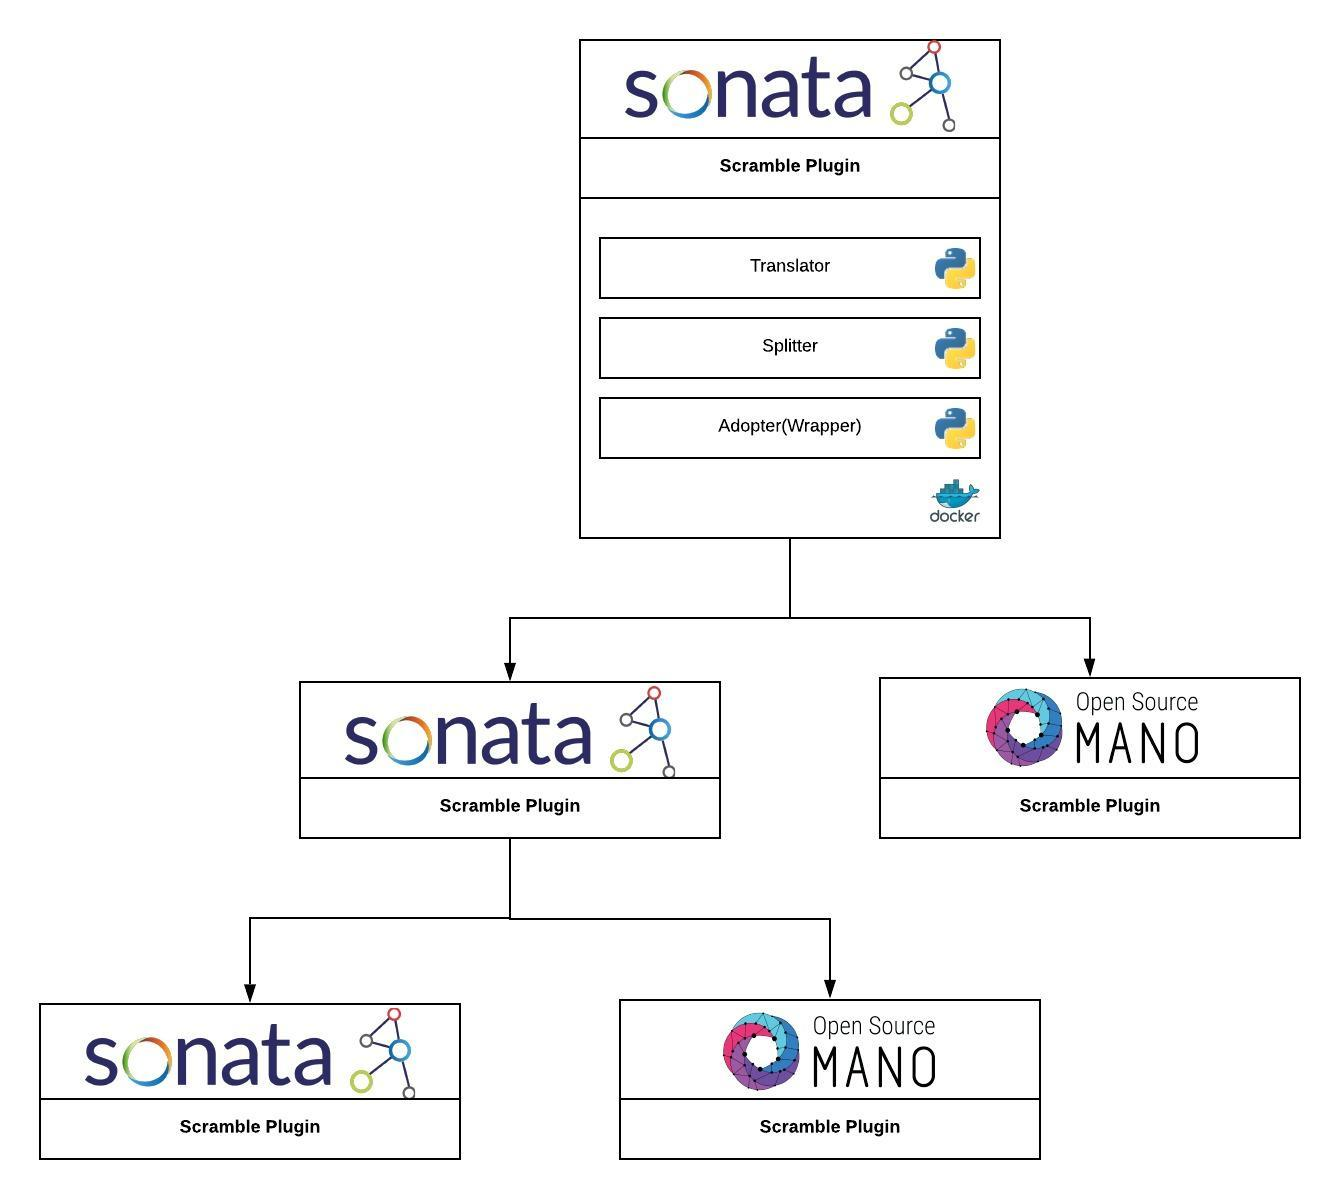
\includegraphics[width=0.7\linewidth]{images/scramblearch}
	\caption{High-level SCrAMbLE Architecture }
	\label{fig:scramblearch}
\end{figure}

\end{frame}



\begin{frame}
\frametitle{References}
\begin{itemize}
	\item Nathan F Saraiva de Sousa, Danny A Lachos Perez, Raphael V Rosa, Mateus AS
	Santos, and Christian Esteve Rothenberg. Network service orchestration: A sur-
	vey. arXiv preprint arXiv:1803.06596, 2018. ii, 10
	
	\item Raul Muñoz, Ricard Vilalta, Ramon Casellas, Ricardo Martínez, Felipe Vicens,
	Josep Martrat, Víctor López, and Diego López. Hierarchical and recursive nfv
	service platform for end-to-end network service orchestration across multiple nfvi
	domains. In 2018 20th International Conference on Transparent Optical Networks
	(ICTON), pages 1–5. IEEE, 2018. 7
    
\end{itemize}
\end{frame}


\bibliography{bib.bib}


\end{document} 